\documentclass[french, 12pt]{report}
\usepackage[latin1, utf8]{inputenc}
\usepackage[T1]{fontenc} 
\usepackage{color}
\usepackage{graphicx}
\usepackage{listings}
\usepackage{amssymb}
\usepackage{amsmath}
\usepackage{pstricks}
\usepackage{enumitem}
\usepackage{multicol}
\usepackage{verbatim}
\usepackage{listings}
\usepackage{tikz}
\usetikzlibrary{arrows,automata}

\setlist[description]{leftmargin=\parindent,labelindent=\parindent}

\newcommand{\cblue}[1]{ \textcolor{blue}{#1}}
\newcommand{\corange}[1]{ \textcolor{orange}{#1}}
\newcommand{\cviolet}[1]{ \textcolor{violet}{#1}}
\newcommand{\crouge}[1]{ \textcolor{red}{#1}}

%% -------------------------  XML
\definecolor{gray}{rgb}{0.4,0.4,0.4}
\definecolor{darkblue}{rgb}{0.0,0.0,0.6}
\definecolor{cyan}{rgb}{0.0,0.6,0.6}

\lstset{
  basicstyle=\ttfamily,
  columns=fullflexible,
  showstringspaces=false,
  commentstyle=\color{gray}\upshape
}

\lstdefinelanguage{XML}
{
  morestring=[b]",
  morestring=[s]{>}{<},
  morecomment=[s]{<?}{?>},
  stringstyle=\color{black},
  identifierstyle=\color{darkblue},
  keywordstyle=\color{cyan},
  morekeywords={xmlns,version,type}% list your attributes here
}
%% ------------------------ END XML

\title{Memo pour l'année}
\author{LAURENT Thomas}
\date{Master 2 informatique 2018}

\begin{document}
\maketitle
\pagebreak
\tableofcontents

\begin{titlepage}
\end{titlepage}
\pagebreak

\part{Fouille de donnée}
\pagebreak

\chapter{Rappel sur les probabilisées}

\begin{description}
\item[Quelques rappels de probabilités]: Soient X et Y deux variables aléatoires discrètes prenant leurs valeurs dans DX={x1,..,xn} et DY={y1,..,ym} respectivement.  
\item[$P(x_i)$] = $\frac{|x_i|}{\sum_{j=1}^n |x_j|}$
\item[] $\sum_{i=1}^n P(x_i) = 1$
\item[$P(x_i | y_i)$] = $\frac{P(x_i,y_i)}{p(y_i)}$
\item[$P(x_i,y_i)$] = $p(x_i) * p(y_i)$ Si X et Y sont indépendantes
\item[règle de chainage $P(x_1,x_2,x_3,...x_n$] = $p(x_1)*p(x_2|x_1)*...*p(x_n|x_{n-1}..x_1)$
\item[distribution conditionnel] $ \forall x in X, \forall y in Y => P(x|y)$
\end{description}

Exemple:
\begin{description}
\item[]: 
\begin{tabular}{ll|ll}
  \hline
  Année & Sexe & \# & \%  \\
  \hline
   M1 & M  & 25  &  25/55   \\
   M1 & F  & 4 &  4/55  \\
   M2 & M  & 25  & 25/55   \\
   M2 & F  & 1  &  1/55  \\
  \hline
\end{tabular}
\item[]
\begin{description}
\item[$P(sexe=M)$] = $P(Sexe=M et Annee=M1) + P(Sexe=M et Annee=M2) = 50/55$
\item[$P(Annee=M2 | sexe=M)$] = $P(Sexe=M et Annee=M2) / P(Sexe=M) = \frac{25}{55} / \frac{50}{55} = \frac{25}{50} = \frac{1}{2}$
\end{description}
\end{description}

\section{Exemple}
\begin{multicols}{2}
[]
\begin{tabular}{ll|l}
  \hline
  $A$&$B$&$P(AB)$\\
  \hline
  $a_1$&$b_1$&.1\\
  $a_2$&$b_1$&.15\\
  $a_1$&$b_2$&.3\\
  $a_2$&$b_2$&.45\\
  \hline
\end{tabular}

\begin{itemize}
\item $P(a_1) = .40$
\item $P(a_1|b_1) = .4$
\item $P(a_1|b_2) = .4$
\item $P(a_2) = .60$
\item $P(a_2|b_2) = .6$
\item $P(a_2|b_2) = .6$
\end{itemize}

\end{multicols}

\chapter{Pré traitement des données}
\section{Nettoyage des données}
\subsection{Caractéristiques descriptives}

Objectifs: Résumer, décrire certains aspects (tendances, variation, dispersion…) des données en utilisant certaines mesures :

\begin{center}
\begin{description}
\item[Moyenne (espérance)]: $\overset{\_}{x}=\frac{1}{n} \sum_{i=1}^n x_i$
\item[Ecart moyen]: $\frac{1}{n} \sum_{i=1}^n |x_i - \overset{\_}{x} |$
\item[Variance]: $v = \frac{1}{n} \sum_{i=1}^n (x_i - \overset{\_}{x} )^2$
\item[Ecart type]: $\alpha x := \sqrt{\frac{1}{n} \sum_{i=1}^n (x_i - \overset{\_}{x} )^2} = \sqrt{\frac{1}{n}(\sum_{i=1}^n x_i^2) - \overset{\_}{x}^2 }$
\item[Médiane]: Valeur se trouvant au milieu d’une série de données ordonnées
\item[Mode]:Valeur la plus fréquente 
\item[Amplitude]:min, max
\end{description}
\end{center}

\section{Normalisation}

\begin{description}
\item[Min-max]: $v_n = \frac{v-v_{min}}{v_{max} - v_{min}}$
\item[Min-max dans l'intervalle [A,B]]: $v_n = \frac{v-v_{min}}{v_{max} - v_{min}} * (B-A) + A$
\item[Z-Score]: $v_n = \frac{v - moyenne}{ecart_type}$
\item[Decimal scaling]: $v_n = \frac{v}{100^j}$
\end{description}

\pagebreak
\chapter{Classification}
\section{Évaluation des classifieurs}
\subsection{Matrice de confusion}
\begin{description}
\item[Percent of correct classification]:
\begin{description}
\item[PCC(\%)]: $ = \frac{N_c}{N_t} * 100$
\item[$N_c$]: nombre d'instances correctement classées
\item[$N_t$]: nombre d'instances testées $(N_t = |D_{test}|)$
\end{description} 
\end{description}

Exemple:\\
\begin{description}
\item[]: $\begin{pmatrix}
  \_  & c1 & c2 & c3 & c4 \\
   c1 & 0  & 1  &  0 & 0  \\
   c2 & 1  & 60 &  0 & 1  \\
   c3 & 0  & 1  & 23 & 0  \\
   c4 & 1  & 0  &  7 & 5  \\
\end{pmatrix}$
\item[Taux d'erreurs]: 100-PCC
\item[PCC(\%)] = $ \frac{0+60+23+5}{100} * 100 = 88\% $ 
\end{description}

\chapter{Arbre de décision}
\section{critères de sélection C4.5}

Construction d’un arbre de décision C4.5  La construction d'un arbre de décision avec C4.5 passe par deux phases:  
\begin{description}
\item[Phase d'expansion]: La construction se fait selon l'approche descendante et laisse croître l'arbre jusqu'à sa taille maximale.  
\item[Phase d'élagage]: Pour optimiser la taille l'arbre et son pouvoir de généralisation, C4.5 procède à l'élagage (pour supprimer les sous-arbres qui ne minimisent pas le taux d'erreurs)
\item[Approche de construction d’un AD]: Partitionner récursivement les données en sous-ensembles plus homogènes  … jusqu’à obtenir des partitions qui contiennent des objets qui appartiennent majoritairement à la même classe. \\
=> Théorie de l’information pour caractériser le degré de mélange, homogénéité, impureté, incertitude…
\item[Théorie de l’information]: Théorie mathématique ayant pour objet l’étude du contenu informationnel d’un message. \\
 Applications en codage, compression, sécurité… 
\item[Entropie]: Mesure la quantité d’incertitude dans une distribution de probabilités.
\end{description}

\subsection{Entropie}
\begin{description}
\item[Entropie]: Mesure la quantité d’incertitude (manque d’information) dans une distribution de probabilités.   Soit X une variable aléatoire discrète prenant ses valeurs dans $DX={x1,..,xn}$. Soit P la distribution de probabilités associée à X.   
\item[$H(X)$] = $- \sum_{i=1}^n p(x_i) * log_2(p(x_i))$
\item[] Par convention, quand $p(x) = 0, 0*log(0) = 0$
\end{description}

Exemple:
\begin{description}
\item[] $\begin{tabular}{|l|c|r|}
  \hline
   X & P(X)\\
  \hline
  x\_1 & 1/3 \\
  x\_2 & 1/3 \\
  x\_3 & 1/3 \\
  \hline
\end{tabular}$
\item[$H(X)$] = $-p(x_1)*log_2(p(x_1))-p(x_2)*log_2(p(x_2))-p(x_3)*log_2(p(x_3))$
\item[$H(X)$] = $-3(\frac{1}{3}*log_2(\frac{1}{3})) = log_2(3) = 1.58$
\end{description}

Autre exemples:
\begin{description}
\item[] $[\frac{1}{2}, \frac{1}{4}, \frac{1}{4}]: H(X) = 1.5$
\item[] $[1, 0, 0]: H(X) = 0$
\item[] $[\frac{1}{2}, \frac{1}{2}]: H(X) = 1$
\end{description}

Propriétés:
\begin{description}
\item[$H(X)$] >= 0
\item[$H(X)$] est maximale pour une distribution uniforme (toutes les valeurs sont équiprobables).
\end{description}

\begin{description}
\item[Entropie conjointe]: L’entropie conjointe de deux variables aléatoires X et Y est l’incertitude relative à ces deux variables conjointement.
\item[$H(X,Y)$] = $- \sum_{i,j=1}^n p(x_i,y_i) * log_2(p(x_i,y_i))$
\item[Exemple]: $[0.2, 0.1, 0.3, 0.4]: H(X,Y) = 1.85$
\end{description}


Critère de sélection: Gain d'information:
\begin{description}
\item[$GAIN(T,A)$] = $Info(T) - Info(T|A)$
\item[Avec $Info(T)$]: Entropie au niveau de T (avant de partitionner)
\item[$Info(T)$] = $-\sum_{c_i} freq(c_i,T)*log_2(freq(c_i,T))$
\item[Avec $freq(c_i,T)$] = $p(c_i) = \frac{|c_i|}{|T|}$
\item[Avec $Info(T|A)$] l'entropie conditionnelle de T une fois partitionné selon les valeurs de l'attribut A.
\item[$Info(T|A)$] = $ \sum_{a_{j \in A}} freq(a_j,T) * Info(T | a_j)$
\end{description}

Critère de sélection: Gain Ration:
\begin{description}
\item[] Le gain d’information favorise les attributs ayant de larges domaines.
\item[] Le ratio de gain utilise le gain d’information avec un facteur pénalisant les attributs ayant des domaines trop larges.
\item[$GainRatio(T,A)$] = $\frac{Gain(T,A)}{Split_Info(T,A)}$
\item[Avec $Split_Info(T,A)$] = $- \sum_{a_{j \in A}} freq(a_j,T)*log_2(freq(a_j,T)) = $Entropie de A.
\end{description}

\section{critères d'arrêt}

\subsection{Critères d'arrêt}
\begin{description}
\item[] Si tout les objets d'une partition appartiennent à une même classes
\item[] Si il n'y a plus aucun attributs à tester
\item[] si le nœud est vide (càd feuille de l'arbre)
\item[] Absence d'apport informationnel (le grain est négatif ou nul)
\end{description}

\subsection{critères d'arrêt: Paramètre utilisateur}
\begin{description}
\item[] Nombre d'objets minimum par feuille
\item[] Taille, profondeur de l'arbre
\item[] Temps de construction de l'arbre
\end{description}

\chapter{Classificateur bayésiens}
\scalebox{0.8}{
\begin{tikzpicture}[->,>=stealth',shorten >=1pt,auto,node distance=8cm,
                    semithick]
  \tikzstyle{every state}=[fill=white,draw=none,text=black]

  \node[state]		   (A)                    {
    \begin{tabular}{ll}
      $ Nuage $ & $p(N)$\\
      \hline
      \hline N=$\bot$ & N=$\top$\\
      \hline 0.5 & 0.5\\
	\end{tabular}\\
  };
  \node[state]         (B) [below left of=A]  {      
     \begin{tabular}{l|ll}
         $ Arroseur$ & $P(A|N) $& $ $ \\
        \hline
        \hline N & A=$\bot$ & A=$\top$\\
        \hline $\bot$ & 0.8 & 0.2\\
         $\top$ & 0.2 & 0.8\\
	  \end{tabular}\\
  };
  \node[state]         (C) [below right of=A] {     
  	\begin{tabular}{l|ll}
        $ Pluie$ & $ P(P|N)$ & $ $ \\
        \hline
        \hline N & P=$\bot$ & P=$\top$\\
        \hline $\bot$ & 0.99 & 0.1\\
        $\top$ & 0.6 & 0.4\\
	  \end{tabular}\\
   };
  \node[state]         (D) [below right of=B] {     
  	\begin{tabular}{ll|ll}
        $ Pelouse$ & $Mouille $ & $ P(M|A,P)$ & $ $ \\
        \hline
        \hline A & P & M=$\bot$ & M=$\top$\\
        \hline $\bot$ & $\bot$ & 0.9 & 0.1\\
        $\bot$ & $\top$ & 0.2 & 0.8\\
        $\top$ & $\bot$ & 0.2 & 0.8\\
        $\top$ & $\top$ & 0.05 & 0.95\\
	  \end{tabular}\\
   };

  \path (A) edge              node {} (B)
            edge              node {} (C)
        (B) edge              node {} (D)
        (C) edge              node {} (D);
\end{tikzpicture}
}
\begin{description}
\item[Calculer] $P(N=\top,P=\top,A=\bot,M=\top)$
\item[$=$] $P(N=\top) * P(P=\top|N=\top) * P(A=\bot|N=\top,P=\top) * \linebreak P(M=\top|N=\top,P=\top,A=\bot)$
\item[$=$] $ .5\ *\ .4\ *\ \frac{P(N=\top,P=\top)P(A=\bot)}{P(N=\top,P=\top)}\ *\ \frac{P(N=\top,P=\top,A=\bot)*P(M=\top)}{P(N=\top,P=\top,A=\bot)}$
\item[$=$] $ .5\ *\ .4\ *\ 1\ *\ $
\end{description}

\pagebreak
\part{Apprentissage automatique par la pratique}
\pagebreak

\chapter{Rappel}
\section{Matrices et calcules sur les Matrices}

\subsection{Addition}

$\left(\begin{array}{cc}
1 & 3 \\ 1 & 0 \\ 1 & 2 \end{array} \right)$
+
$\left(\begin{array}{cc}
0 & 0 \\ 7 & 5 \\ 2 & 1 \end{array} \right) $
=
$\left(\begin{array}{cc}
1+0 & 3+0 \\ 1+7 & 0+5 \\ 1+2 & 2+1 \end{array} \right) $
=
$\left(\begin{array}{cc}
1 & 3 \\ 8 & 5 \\ 3 & 3 \end{array} \right) $

\subsection{Multiplication}

$\begin{array}{c@{\ }c}
&
\left(\begin{array}{cc}
5 & 6 \\ 7 & 8 \end{array} \right) \\[0.5cm]
\left(\begin{array}{cc}
1 & 2 \\ 3 & 4 \end{array} \right)
&
\left(\begin{array}{cc}
19 & 22 \\ 43 & 50 \end{array} \right)
\end{array}$

$(1 * 5) + (2 * 7) = 19$

\subsection{Transposer}

$\left(\begin{array}{ccc}
1 & 3 & 5 \\ 2 & 4 & 6 \end{array} \right) $
= 
$\left(\begin{array}{cc}
1 & 2 \\ 3 & 4 \\ 5 & 6 \end{array} \right) $

\subsection{Inverse}
\begin{description}
\item[Soit une matrice 2x2 comme]:
$\left(\begin{array}{ccc}
a & b \\ c & d \end{array} \right) $
\item[Soit Determinant D] = ad - bc
\item[Si D != 0 alors il existe une matrice inverse égal à]:
$ \frac{1}{D} \left(\begin{array}{ccc}
d & -b \\ -c & a \end{array} \right) $
\end{description}

\chapter{Algorithms Learn a Mapping From Input to Output}
\section{linear ML algorithms}

\begin{description}
\item[] Simplifier les processus d'apprentissage et réduire la fonction sur ce qu'on connait
\item[Soit ]: B0 + B1X1 + B2X2 + B3X3 = 0
\item[] Où B0,B1,B2,B3 sont les coefficients présent sur l'axe des ordonnées.
\item[] Et X1,X2,X3 sont les valeurs en Input.
\end{description}

\section{Supervised machine learning}
L'apprentissage supervisé peut se diviser en 2 partis
\begin{description}
\item[Classification]: Quand les variables en sortie sont des Classe $(Vert, Carré, Homme)$
\item[Regression]: Quand les variables en sortie sont des valeur numérique $(euro, poids, quantités)$
\end{description}

\section{Unsupervised machine learning}
Les problèmes de l'apprentissage non supervisé sont:
\begin{description}
\item[Clustering]: L'art de faire des paquet d'éléments qui ont des points commun, comme regrouper les clients par paquet de choses qu'ils ont le plus en commun.
\item[Association]: Associer des règles d'apprentissage pour décrire une portion du data, comme une personne qui a acheté un item A et qui est aussi tenté par acheter un item B
\end{description}

\section{semi-supervised machine leaning}
L'apprentissage semi supervisé c'est avoir un bonne quantité de données en input X, et un peu de data avec le label Y.

\section{Overview of dias and variance}
La prédiction des erreurs pour les algorithmes sont regroupé en 3 points:
\begin{description}
\item[Bias Error]:  Simplifier l'hypothèse fait par le modèls pour faire une fonction d'apprentissage plus facile.
\item[Variance Error]: Et la quantité estimé par la fonction visé qui changera via un différent ensemble de data utilisé.
\item[Irreductible Error]: Ne peut pas être réduit
\end{description}

\chapter{Overfitting and Underfitting}
\section{Overfitting}
L'overfitting intervient lorsque le modèle sur apprend des connaissances,
Lorsque l'on sur apprend nous prenons en compte les points plus éloigné de la droite de la fonction.\\
On peut illustrer l'overfitting en codant un algorithme qui prend en compte les points bleu et rouges de la figure $\textit{ap-linear-regression\_1}$ ce dessous.\\

\section{Underfitting}
C'est l'inverse de l'overfitting, pas assez de données pour pouvoir généraliser le base de connaissance.\\
\pagebreak
\chapter{Linear Algorithms}

Soit X l'ensemble des variables indépendantes sur l'axe des l'abscisse et
Y l'ensemble des variable dépendantes sur l'axe des ordonnée.

\section{Régression linéaire}
Étant donné un plan à deux dimensions où l'abscisse contient les point d'entrée X et l'ordonnée contient les points de sortie Y, et un nouage de points précédaient acquitté de tout point éloigné du nuage.

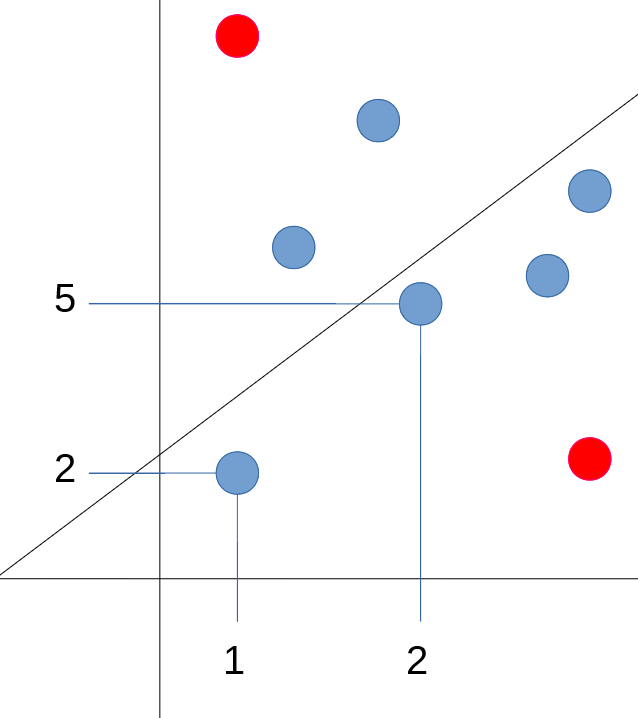
\includegraphics[scale=0.3]{img/ap-linear-regression_1.png}
$Figure ap-linear-regression_1$

\begin{description}
\item[Avec]: y  = $\beta_0 + \beta_1 x$
\item[Pour un hyperPlan (3d)]: y = $\beta_0 + \beta_1 x_1 + \beta_2 x_2$
\item[$P-I_n$]: y = $\beta_0 + \beta_1 x_1 + ... \beta_n x_n$
\end{description}

Exemple:
\begin{description}
\item[5] =  $\beta_0 + 2 * \beta_1$
\item[2] =  $\beta_0 + 1 * \beta_1$
\end{description}

\pagebreak
\section{Least squares linear regression}
Calculer la régression linéaire avec la méthode Least squares:\\
Soit:
\begin{description}
\item[X] = $[1,2,3,4,5]$ les variables indépendantes d'axe abscisse
\item[Y] = $[2,4,5,4,5]$ les variables dépendantes d'axe ordonnée
\item[Calculons] $y = \beta_0 + \beta_1 x$
\end{description}
Calcule de la moyenne de X et Y:
\begin{description}
\item[Xm] = $ \sum x_i \in X$ = 3
\item[Ym] = $ \sum y_i \in Y$ = 4
\end{description}
Toutes ligne de régression doivent passer par le point (Xm,Ym).\\
Calculer tout les écarts des $x_i \in X$ par rapport à Xm (resp Y):\\

\begin{tabular}{ll|l|l|l|l}
  \hline
  X  & Y & $X - Xm$ & $Y - Ym$ & $(X-Xm)^2$ & $(X-Xm)(Y-Ym)$\\
  \hline
  1 & 2 & -2 & -2 & 4 & 4\\
  2 & 4 & -1 & 0  & 1 & 0\\
  3 & 5 & 0  & 1  & 0 & 0\\
  4 & 4 & 1  & 0  & 1 & 0\\
  5 & 5 & 2  & 1  & 4 & 2\\ 
  \hline
\end{tabular}

\begin{description}
\item[$Calculer \beta_1$]:
\item[$ \beta_1 $] = $ \frac{ \sum (X-Xm)(Y-Ym)}{ \sum (X-Xm)^2}$ = $\frac{6}{10}$ = $.6$
\item[$ \beta_0 $]: $Ym = \beta_0 + \beta_1 * Xm$ : $4 = \beta_0 + .6 * 3$ : $4= \beta_0 + 1.8$ : $\beta_0 = 2.2$
\end{description}
\pagebreak
\section{Gradient Descent}
Soit:
\begin{description}
\item[X] = $[1,2,4,3,5]$
\item[Y] = $[1,3,3,2,5]$
\item[i] = une variable qui itère les éléments de X et Y en bouclant à l'infini.
\end{description}
Une initialisation comme:
\begin{description}
\item[$\beta_0$] = 0
\item[$\beta_1$] = 0
\item[$\alpha$] = donnée en énoncé (pour l'exemple égal à 0.01)
\end{description}
Et des fonctions définit tel que:
\begin{description}
\item[error] = $(\beta_0 + \beta_1 * X[i]) - Y[i]$
\item[$\beta_{0_{+1}}$] = $\beta_0 - \alpha * error$
\item[$\beta_{1_{+1}}$] = $\beta_1 - \alpha * error * X[i]$
\end{description}

En appliquant l'algorithme des calcules des $\beta_i$:\\
\begin{tabular}{l|l|l|l|l|l}
  \hline
  $ i $ & $ X[i] $ &  $Y[i] $ &  $error $ & $ \beta_0 $ & $ \beta_1 $\\
  \hline
  0 & 1 & 1 & -1 & 0.01 & 0.01 \\
  1 & 2 & 3 & -2.97 & 0.06 & 0.03\\
  2 & 4 & 3 & -1.77 & 0.18 & 0.06\\
  3 & 3 & 2 & -1.61 & 0.22 & 0.08\\
  4 & 5 & 5 & -4.35 & 0.44 & 0.12\\
  0 & 1 & 1 & -0.42 & 0.45 & 0.13\\
  1 & 2 & 3 & -2.28 & 0.49 & 0.49\\
  \hline
\end{tabular}
\pagebreak
\chapter{Logistic Regression}
\section{Logistic function}

Soit:
\begin{description}
\item[t] $\in \Re[0,1]$ égal à $\beta_0 + \beta_2 * x$
\end{description}

La fonction de logique de régression, les valeur d'entrée X sont combiné en utilisant les coefficient de valeur pour prédire une sortie Y. Cette sortie sera une valeur binaire.

\begin{description}
\item[$p(x)$] = $ \frac{1}{1 + e^{-(P-I_n)}}$
\item[Note]: $p(x)$ peut être interprété comme une fonction de probabilité $P(X) = P[Y=1 | X)$.
\item[$\beta_0 + \beta_1 * x$] = $ ln(\frac{P(x)}{1 - P(x)})$ aussi appelé odds.
\end{description}

\section{Linear Discriminant Analysis}
L'analyse discriminante linéaire fait partie des techniques d'analyse discriminante prédictive, il s'agit de prédire l'appartenance d'un individu à une classe prédéfinie à partir de ses caractéristiques mesurées à l'aide de variables prédictives.\\
A notre disposition, un échantillon de $n$ observations réparties dans $\Bbbk$ groupes d'effectifs $n_{\Bbbk}$.\\
\begin{description}
\item[Noté $Y$] les variables prédire $\{y1, ... y_{\Bbbk}\}$
\item[$J$] variables prédictives $X = (X_1, ... X_j)$
\item[$\mu_{\Bbbk}$] la moyenne (ou $\textit{mean}$ en anglais) valant $lambda(list) -> \frac{\sum list[i]}{taille(list)}$
\item[$\sigma^2$] la variance de toutes les classes $\frac{\sum_{i=1}^n (x_i - \mu_{\Bbbk})^2}{n - \Bbbk}$
\item[la fonction discriminante pour la classe $\Bbbk$ avec $x$ donné] $D_{\Bbbk} (x) = x * \frac{\mu_{\Bbbk}}{\omega^2} - \frac{\mu_{\Bbbk}^2}{2x\omega^2} + ln(P(k))$
\item[Où $P(k)$] vaut la probabilité appliqué aux valeurs de $Y$
\end{description}

\subsection{la règles bayésienne}
L'objectif est de produire une règle d'affection $X(\omega) \rightarrow Y(\omega)$ qui permet de prédire, pour une observation $\omega$ donné, sa valeur associé de $Y$ à partir des valeurs prises par $X$. via une probabilité\\
\begin{description}
\item[$P(Y=y_{\Bbbk})$] = $\frac{P(Y=y_{Bbbk})*P(X|Y=y_{\Bbbk})}{\sum_{i=1}^{\Bbbk} P(Y=y_i)*P(X|Y=y_i)}$
\item[Où $P(Y=y_{\Bbbk})$] est la probabilité à $priori$ d'appartenance à une classe
\item[$P(X|Y=y_{\Bbbk})$] représente la fonction de densité des X conditionnellement à la classe $y_{\Bbbk}$
\end{description}

\pagebreak
\chapter{Outils formel}
\pagebreak

\section{Logique classique des propositions}
\subsection{Vocabulaire}

\begin{description}
\item[Déduction] $\models \alpha$ ssi$ \neg \alpha$ est contradictoire
\item[Absurde] $\phi$ est contradictoire ssi $\neg \phi$ est valide
\item[DAG]: Un graphe dirigé acyclique
\item[Taille(Arbre)] = $\{ tout les symboles + connecteurs \}$
\item[Var(Arbre)] = $\{ Toutes les feuilles \}$
\item[Sous formules(Arbres)] = $\{ T + \cup_{i=0}^k SousFormules(Arbre_i) \}$
\item[Interprétation]: $\omega$ de $PROP_{ps}$ est une application de PS dans ${0.1}$
\item[Sémantique]: $[| \phi |](\omega)$ d'une formule $\phi$ de $PROP_{ps}$ dans l'interprétation $\omega$ est une élément de ${0.1}$ définit inductive ment par:
\begin{description}
\item[$si \phi \in PS$] alors $[|\phi|](\omega) = \omega(\phi)$
\item[$si \phi = cX_1 ... X_n$] alors $[|\phi|](\omega) = C_F([|x_1|](\omega) ... [|x_n|](\omega))$
\end{description}
\item[$\omega $ satisfait $ \phi$] noté $\omega \models \phi $ssi$ [|\phi|](\omega) = 1$
\item[Lorsque $\omega \models \phi$] on dit que $\omega$ est un modèle de $\phi$
\item[on note $\eta(\phi)$] l'ensemble des modèles de $\phi$
\item[$\omega \in PROP_{ps}$ est valide] noté $\models \phi$, ssi toute interprétation$ \omega de PROP_{ps}$ satisfait$ \phi$
\item[$phi \equiv \psi$] sont logiquement équivalents ssi$ phi \models \psi$ et $psi \models \phi$
\end{description}

\subsection{Propriétés de l'opérateur Models}

\begin{description}
\item[$a \models b$] $=== M(a) \subseteq M(b)$
\item[Réflexivité]: $\phi \models \phi$
\item[Équivalence à gauche]: si $\phi \equiv \theta $et$ \phi \models \psi $alors$ \theta \models \psi$
\item[Affaiblissement à droite (transitivité)]: si$ \phi \models \psi $et$ \psi \models \theta $alors$ \phi \models \theta$
\item[Coupure]: si$ \phi \wedge \psi \models \theta $et$ \phi \models \psi $alors$ \phi \models \theta$ : $=== (A \cup B) \subseteq C ssi A \subseteq C \cap B \subseteq C$
\item[] 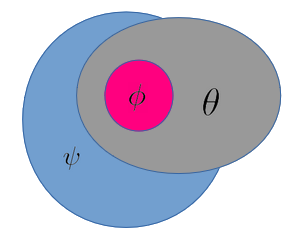
\includegraphics[scale=0.3]{img/of-coupure.png} 
\item[Ou]: $\phi \vee \psi \models \theta $ssi$ \phi \models \theta $et$ \psi \models \theta$
\item[] 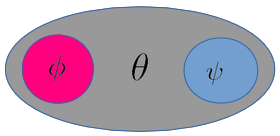
\includegraphics[scale=0.3]{img/of-ou.png}
\item[Monotonie]: si $\phi \models \theta $alors$ \phi \wedge \psi \models \theta$
\item[] 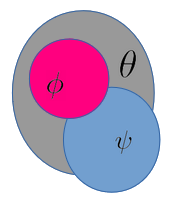
\includegraphics[scale=0.3]{img/of-monotomie.png}
\end{description}

\subsection{Ensemble de connecteurs fonctionnellement complet}
\begin{description}
\item[On dit qu'un ensemble est fonctionnellement complet] si avec que les connecteurs de cette ensemble on peut exprimer toutes les formules d'un monde.
\item[$\{\neg, \wedge\}$] est fonctionnellement complet pour la logique propositionnel classique
\item[] Il en va de même pour $\{\neg, \vee\}, \{vrai, \wedge, \bigoplus\}, \{\neg, \Rightarrow\} ou \{NAND\}$

\begin{description}
\item[Suppression des fils équivalent]: Soit un arbre D ayant comme sous arbre plus d'une fois le nœud $\alpha = (\top X \top)$, $\alpha$ peut être remplacé par $(\top)$ tout en concevant les modèles de D.
\item[fusion des nœuds]: Soit un arbre D ayant comme sous arbre les nœuds $(a B c)$ et $(a` B` c`)$ et $a = a`, b = b`, c = c`$ alors on peut faire relier les deux branches menant vers ces nœuds vers le même sous arbre.
\end{description}
\end{description}

\subsection{Preuve par induction structurelle sur un ensemble de connecteurs non fonctionnellement complet}

Soit $ \forall P \in \{ \wedge, \vee \}_{ps}$, vérifier P:
\begin{description}
\item[Cas de base $\varphi \in PS$]: $1^\rightarrow (\varphi) = 1$ donc $1^\rightarrow$ constitue un modèle de $\varphi$
\item[Étape inductive]: 
\begin{description}
\item[$\varphi$ s'écrit]: $[\alpha \wedge \beta]$ ou $[\alpha \vee \beta]$
\item[] Avec $\alpha, \beta \in \{ \wedge, \vee \}_{ps}$
\item[] Par hypothèse d'induction, $\alpha et \beta$ vérifient P.
\item[] Il ne reste plus qu'a montrer que $\varphi$ vérifie P.
\item[] $[| \alpha \vee \beta |)(1^\rightarrow)$ = $\vee \models ([|\alpha |)(1^\rightarrow), [|\beta |)(1^\rightarrow))$ = $\vee \models (1,1)$ = $1$
\item[] $[| \alpha \wedge \beta |)(1^\rightarrow)$ = $\wedge \models ([|\alpha |)(1^\rightarrow), [|\beta |)(1^\rightarrow))$ = $\wedge \models (1,1)$ = $1$
\item[] donc $x \wedge \neg x$ ne vérifie pas  $P: [| x \wedge \neg x|)(1^\rightarrow) = 0$
\end{description}
\end{description}

\subsection{Décomposition de Shannon}
\begin{description}
\item[On note $\phi [x \leftarrow 0 ) $ ] la formule obtenue en substituant dans $\phi$ la constante faux à toutes les occurrences du symbole propositionnel x.
\item[On note $\phi [x \leftarrow 1 ) $ ] la formule obtenue en substituant dans $\phi$ la constante vrai à toutes les occurrences du symbole propositionnel x.
\end{description}

La décomposition de Shannon de $\phi$ suivant x est la formule:
\begin{description}
\item[] $(\neg x \wedge \phi [x \leftarrow 0]) \vee (x \wedge \phi [x \leftarrow 1])$
\end{description}

\pagebreak
\subsection{Arbre de Shannon, ROBDD}
Étant donnée un ordre strict total $x_1 < x_2 < x_3$ sur $Var(\phi ) = \{x_1, ..... X_n\}$\\
Et une formule $\phi = (\neg x_1 \wedge x_2) \vee ( \neg x2 \wedge x_3)$\\\
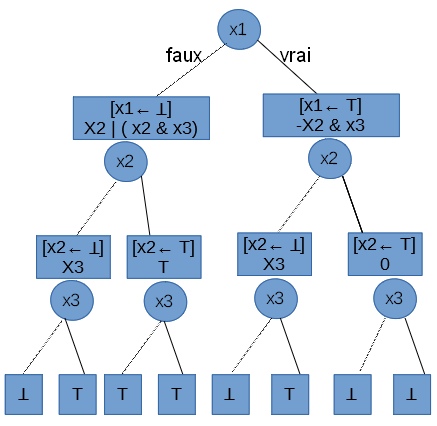
\includegraphics[scale=0.4]{img/of-arbre-shannon_1.png} \\
L'ensemble des modèles de $\phi$ sont toutes les interprétation où la feuille vaut la valeur $T$.

\subsubsection{Remplacement ou vérifonctionnalité}
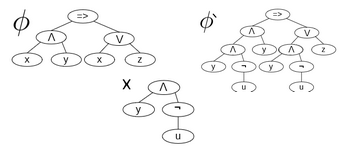
\includegraphics[scale=0.8]{img/of-remplacement.png} \\

$\phi \equiv \phi^{`}$ quelque soit la valeur de x (vrai ou faux).

\subsubsection{Substitution}
Soit un arbre $D$ ayant comme nœud un sous arbre du type infixe $\alpha = (x \Rightarrow y)$ et un sous arbre de substitution $\beta = (\neg x \Rightarrow \neg y)$\\
$(D^{`} = D_{\alpha \leftarrow \beta} \equiv D$)\\

\subsection{Notion de impliquant premier }
Les impliquant premier sont des sous formules des formules original tel que ces sous formules soit plus petite que la formule d'origine elle conserve les même modèles:\\
En circuit combinatoire les algo sont appelé  Table de Karnaugh ou Quine-McCluskey.

\subsubsection{Table de Karnaugh}
Appliquer l'algorithme avec la formule S = $\neg a b \neg c d + a \neg b \neg c \neg d + b \neg d$\\

\begin{tabular}{l|l|l|l|l}
  \hline
  S & $\neg a \neg b$ & $\neg a b$ & $ab$ & $a \neg b$\\
  \hline
  $\neg c \neg d$ & X & X & X & X \\
  $ \neg c d $ & $ $ & X & X & $ $ \\
  $cd$ & $ $ & X & X & $ $ \\
  $c \neg d$ & X & X & X & X \\
  \hline
\end{tabular}\\

les impliquant premier de S sont $b \neg d$\\

\subsubsection{Calcule arithmétique}
En logique, les impliquant premier sont calculer que à partir d'une formule en mode CNF transposé en DNF et ensuite détransposé en CNF.

\begin{description}
\item[$\phi$] = $(a \wedge b \wedge c) \vee ( \neg b \wedge c)$
\item[$\phi$] = $(a \vee \neg b) \wedge (a \vee c) \wedge ( b \vee \neg b) \wedge (b \vee c) \wedge (c \vee  \neg b ) \wedge (c \vee c)$
\item[$\phi$] = $(a \vee \neg b) \wedge (a \vee c) \wedge (b \vee c) \wedge (c \vee \neg b) \wedge c$
\item[$\phi$] = $(a \vee \neg b) \wedge c$
\item[$\phi$] = $(a \wedge c) \vee (\neg b \wedge c)$ sont les impliquant premier.
\end{description}

Via une table de Karnaugh:\\
\begin{tabular}{l|l|l|l|l}
  \hline
  $\phi$ & $\neg a \neg b$ & $\neg a b$ & $ab$ & $a \neg b$\\
  \hline
  $\neg c$ & $ $ & $ $ & $ $ & $ $ \\
  $c$ & X & $ $ & X & X \\
  \hline
\end{tabular}\\
Égal à $(a \wedge c) \vee (\neg b \wedge c)$.

\subsection{Système de Hilbertien}

gg

\subsection{Forte complétude OU théorème de finitude}

g

\pagebreak

\part{Recherche Opérationnel}
\pagebreak
\chapter{Introduction à la PL}\pagebreak

Construire une modèle linéaire, c'est donc:
\begin{description}
\item[identifier] les variables de décision du problème
\item[déterminer]: la fonction objectif du modèle
\item[déterminer]: les contraintes du modèle 
\end{description}

\section{Modèle linéaire continus à 2 variables}
Soit le modèle linéaire suivantes:
\begin{description}
\item[Déterminer] $(x,y) \in \Im^2$
\item[Minimisant] $z = 1000x + 1200y$
\item[sous les contraintes]:
\begin{description}
\item[] $(1) 8x + 4y \leq 160$
\item[] $(2) 4x + 6y \leq 120$
\item[] $(3) x \leq 34$
\item[] $(4) y \leq 14$
\item[] $(5) 0 \leq x$
\item[] $(6) 0 \leq y$
\end{description}
\end{description}

\subsection{Recherche de solutions}
Après avoir tracé graphiquement tout les points:\\
Pour chaque contrainte, tracer la droite et repérer le demi plan des solution: exemple pour (5) et (6), x et y doivent être supérieurs ou égal à 0, d'où le demi plan des solution sont toutes les valeurs positives.\\
La partie En vert représente la région admissible, quelque soit le point choisis dans ce vert, aucune contrainte ne sera violé.\\
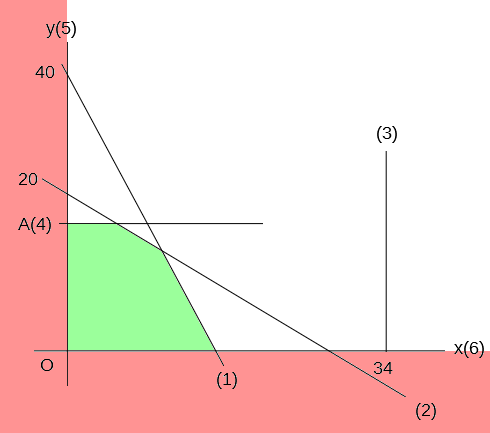
\includegraphics[scale=0.55]{img/ro-pl-2var_0.png} 
\subsection{recherche de la solution optimal}

Changer l'équation $z$ tel que $z$ soit égal à $0$
\begin{description}
\item[$z$] = $1000x + 1200y$ = $0$ = $1000*(1200) + 1200 *(-1000)$
\end{description}
Traçons la droite $(0,0)$, $(1200,-1000)$
\begin{description}
\item[Un point extrême]: est un point se trouvant sur l'intersection de 2 contraintes et étant dans la zone admissible.
\item[L'altitude]: est la droite (rouge) la plus haute touchant un point extrême, ce point sera le vecteur $(x,y)$ le plus optimal pour $z$.
\item[] Les droites rouges doivent être toutes parallèles.
\end{description}
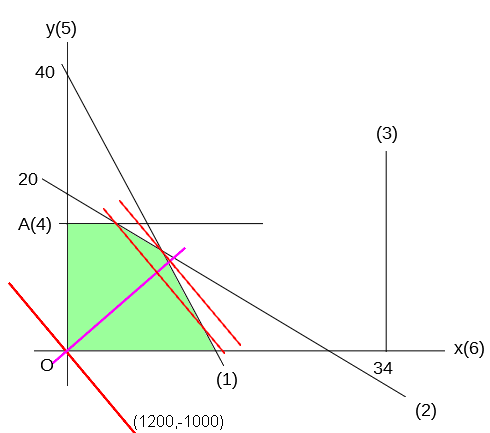
\includegraphics[scale=0.55]{img/ro-pl-2var_1.png} \\
Dans cette exemple le point (15,10) est le point extrême maximal pour l'équation z.\\
\pagebreak
\chapter{Le simplexe}\pagebreak
Soit le modèle linéaire suivantes:
\begin{description}
\item[Déterminer] $(x,y) \in \Im^2$
\item[Maximisant] $Z = 3x + 7y$
\item[sous les contraintes]:
\begin{description}
\item[] (1) $ -x + y \leq 3$
\item[] (2) $ y \leq 8$
\item[] (3) $ 2x - y \leq 28$
\item[] (5) $ 0 \leq x$
\item[] (6) $ 0 \leq y$
\end{description}
\end{description}

\section{Initialisation du simplexe}
Pour chaque expression du type $(1)(2)(3)$ intégrer un $e_i$ pour la transformer en équation.\\
On appel les $e_1$ des variables d'accumulation, Ce qui fait\\
\begin{description}
\item[Déterminer] $(x,y,e_1,e_2,e_3) \in \Im^5$
\item[Maximisant] $Z = 3x + 7y$
\item[sous les contraintes]:
\begin{description}
\item[] (1) $ -x + y + e_1 = 3$
\item[] (2) $ y + e_2 = 8$
\item[] (3) $ 2x - y + e_3 = 28$
\item[] (5) $ 0 \leq x$
\item[] (6) $ 0 \leq y$
\item[] (7) $ e_1,e_2,e_3 \geq 0$
\end{description}
\end{description}

\section{Canonicité du modèle}
Soit les valeurs (pour la première itération)
\begin{description}
\item[Hors Base] $(x,y)$
\item[Base] $(e_1,e_2,e_3)$
\end{description}

Un modèle est canonique que si:
\begin{description}
\item[si toutes les variables de Base] ne sont pas dans Z.
\end{description}

\section{Solution admissible}
\begin{description}
\item[] (1) $-x + y + e_1 = 3$
\item[] (2) $x - e_1 + e_2 = 5$
\item[] (3) $3x - e_1 + e_3 = 25$
\item[Variable hors base] = $x,e_1$
\item[Variable Base] = $y,e_2,e_3$
\item[Avec comme solution admissible] $A\ Deduire (x,y,e_1,e_2,e_3)$
\end{description}
\ \\
Pour toute variable présente dans l'ensemble $Hors\ base$ la valeur admissible est égal à $0$\\
Donc solution admissible = $(0, y, 0, e_2, e_3)$\\
Les 3 dernières valeurs sont les résultat des équations (soit $3$, $5$ et $25$).\\
Pour chaque équation nous lisons les termes de droit à gauche et ignorons ceux qui sont dans l'ensemble $Hors\ Base$:\\
Donc solution admissible = $(0, 3, 0, 5, 25)$\\

\section{Exemple simple Premier itération}
\subsection{Choix de la variable entrante}
\begin{description}
\item[Gain marginale] prendre la variable non négatif ayant le plus haut coefficient.
\end{description}
$(x,y)$ sont deux choix possible, le tout est de choisir une bonne heuristique, comme celle du meilleur gain marginale, ou via la comparaison (en mode graphique):\\
$Y$ sera choisit, donc $Y$ sera notre variable entrante.\\

\subsection{Choix de la variable sortante}
Pour chaque résultat d'équation, le diviser par sa valeur de $Y$ (le résultat devant être positif sinon l'ignorer)\\

\begin{description}
\item[] $ -x + y + e_1 = 3$ donne $\frac{3}{\crouge{1}} = 3$ (1 car $y$ = $1*y$)
\item[] $ y + e_2 = 8$ donne $\frac{8}{1} = 8$
\item[] $ 2x - y + e_3 = 28$ donne $\frac{28}{1} = 28$
\end{description}
Prendre le minimum des variables, donc se sera $3$.\\
la variable présente dans la Base sera prise comme variable sortante, dans notre cas $e_1$.\\
\pagebreak
\subsection{pivotage}
On choisis l'équation associé à la variable $e_1$ pour définir la variable entrante $y$.\\
On n'a:
\begin{description}
\item[$y$] = $\frac{1}{\crouge{1}}*(x - e_1 + 3)$
\end{description}

Puis on crée les nouvelles équations via le nouveau $y$:
\begin{description}
\item[$Z = 3x + 7y$] devient
\begin{description}
\item[$Z$] = $3x + 7(x - e_1 + 3)$
\item[$Z$] = $10x - 7e_1 + 27$
\end{description}
\item[$x - e_1 = 3$] est déjà normalisé
\item[$y + e_2 = 8$] devient
\begin{description}
\item[$8$] = $x -e_1 + 3 + e_2$
\item[$5$] = $x - e_1 + e_2$
\end{description}
\item[$2x - y + e_3 = 28$] devient
\begin{description}
\item[$28$] = $2x + (x - e_1 + 3) + e_3$
\item[$25$] = $3x - e_1 + e_3$
\end{description}
\end{description}
\subsection{Nouveau modèle}
\romodel{$(x,y,e_1,e_2,e_3) \in \Im^5$}
        {Maximisant}{$Z = 10x - 7e_1 + 21$}
        {$x,e_1$}{$y,e_2,e_3$}{$(0,3,0,5,25)$}{$21$}
        {\begin{description}
\item[] (1) $-x + y + e_1 = 3$
\item[] (2) $x - e_1 + e_2 = 5$
\item[] (3) $3x - e_1 + e_3 = 25$
\item[] (5) $ 0 \leq x$
\item[] (6) $ 0 \leq y$
\item[] (7) $ e_1,e_2,e_3 \geq 0$
\end{description}
}

A ne pas oublier de vérifier la canonicité du modèle.\\

\section{Exemple simple Seconde itération}
\subsection{Choix de la variable entrante}
$X$ sera choisit, donc $X$ sera notre variable entrante.\\

\subsection{Choix de la variable sortante}
\begin{description}
\item[] $\frac{5}{\crouge{1}} = 5$
\item[] $\frac{25}{3} = 8.3$
\end{description}
Prendre le minimum des variables, donc se sera $5$, donc $e_2$.\\

\subsection{pivotage}
\begin{description}
\item[$x$] = $\frac{1}{\crouge{1}}*(e_1 - e_2 + 5)$
\end{description}

Puis on crée les nouvelles équations via le nouveau $y$:
\begin{description}
\item[$Z = 10x - 7e_1 + 27$] devient
\begin{description}
\item[$Z$] = $10(e_1 - e_2 + 5) - 7e_1 + 27$
\item[$Z$] = $3e_1 - 10e_2 + 71$
\end{description}
\item[$-x + y + e_1 = 3$] devient
\begin{description}
\item[$3$] = $-(e_1 - e_2 + 5) + y + e_1$
\item[$8$] = $y + e_2$
\end{description}
\item[$3x - e_1 + e_3 = 25$] devient
\begin{description}
\item[$25$] = $3(e_1 - e_2 + 5) -e_1 + e_3$
\item[$10$] = $2e_1 - 3e_2 + e_3$
\end{description}
\end{description}

\subsection{Nouveau modèle}
\romodel{$(x,y,e_1,e_2,e_3) \in \Im^5$}
        {Maximisant}{$Z = 3e_1 - 10x + 71$}
        {$e_2,e_1$}{$y,x,e_3$}{$(5,8,0,0,10)$}{$71$}
        {\begin{description}
\item[] (1) $y + e_2 = 8$
\item[] (2) $x - e_1 + e_2 = 5$
\item[] (3) $2e_1 - 3e_2 + e_3 = 10$
\item[] (5) $ 0 \leq x$
\item[] (6) $ 0 \leq y$
\item[] (7) $ e_1,e_2,e_3 \geq 0$
\end{description}
}

A ne pas oublier de vérifier la canonicité du modèle.\\

\section{Exemple simple, troisième itération}
\subsection{Variable entrante et sortante}
\rovarinout{$e_1$}{$e_3$}
  {$\frac{8}{0}$ est NULL}
  {$\frac{5}{1}$ car négatif}
  {$\frac{10}{2} = 5$}

\subsection{Nouveau modèle}
\romodel{$(x,y,e_1,e_2,e_3) \in \Im^5$}
        {Maximisant}{$Z = 86 - \frac{11}{2}e_2 - \frac{3e_3}{2}$}
        {$e_2,e_3$}{$y,x,e_1$}{$(10,8,5,0,0)$}{$86$}
        {\begin{description}
\item[] (1) $- \frac{1}{2}e_2 + \frac{e_3}{2} + e1 = 10$
\item[] (2) $e_2 + y = 8$
\item[] (3) $e_1 - \frac{3}{2}e_2 + \frac{e_3}{2} = 5$
\item[] (5) $ 0 \leq x$
\item[] (6) $ 0 \leq y$
\item[] (7) $ e_1,e_2,e_3 \geq 0$
\end{description}
}
\section{Exemple simple, dernière itération}
Stop car $e_2$ et $e_3$ sont inférieur à 0 dans $Z$.

\chapter{Simplexe à deux phases}\pagebreak
Soit le modèle suivant:
\begin{description}
\item[Déterminer] $(x,y) \in \Im^2$
\item[Maximisant] $Z = 2x + 3y$
\item[sous les contraintes]:
\begin{description}
\item[] (1) $x + y \leqslant 4$
\item[] (2) $x + 2y \leqslant 5$
\item[] (3) $4x -y \geqslant 2$
\item[] (4-5) $x,y \geqslant 0$
\end{description}
\end{description}

Lorsque le sens de l'équation est $\leqslant$ il faut ajouter une variable $e_i$, dans le cas des équations $\geqslant$
il faut ajouter une variable d'excédant $a$ dans la contrainte concerné et instaurer $Z$ à $- a$\\
La représentation graphique ci dessous:\\
\begin{center}
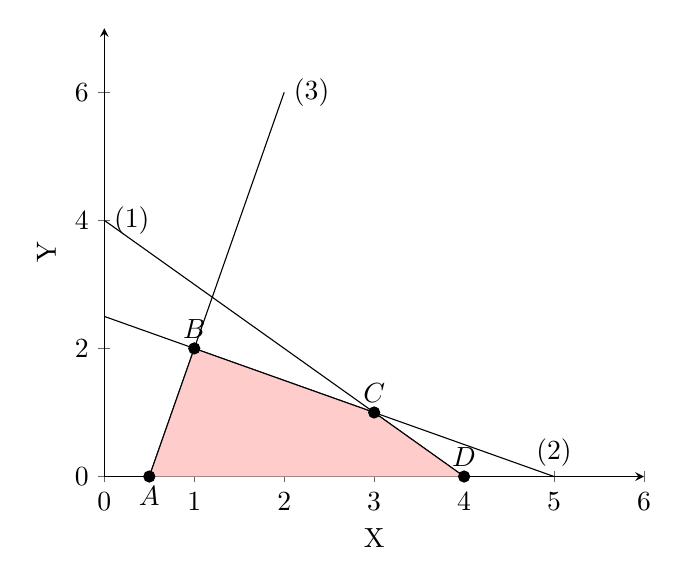
\begin{tikzpicture}
  \begin{axis} [
      xlabel     = X, % label x axis
      ylabel     = Y, % label y axis
      axis lines = left, %set the position of the axes
      clip       = false, 
      xmin       = 0,
      ymin       = 0,
      xmax       = 6,
      ymax       = 7,
    ]
    \addplot [color=black] coordinates { (4,0)(0,4) } node[right] {$(1)$};
    \addplot [color=black] coordinates { (0,2.5)(5,0) } node[above] {$(2)$};
    \addplot [color=black] coordinates { (0.5,0)(2,6) } node[right] {$(3)$};
    
    \addplot [only marks, mark=*, color=black] coordinates { (0.5,0) } node[below] {$A$};
    \addplot [only marks, mark=*, color=black] coordinates { (1,2) } node[above] {$B$};
    \addplot [only marks, mark=*, color=black] coordinates { (3,1) } node[above] {$C$};
    \addplot [only marks, mark=*, color=black] coordinates { (4,0) } node[above] {$D$};
    
    \addplot [color=black, style={fill=red!20}] coordinates { (0.5,0)(1,2)(3,1)(4,0) };
  \end{axis}
\end{tikzpicture}
\end{center}
\section{Première phase du simplexe à deux phases}
Pour toutes expression sous la forme $ A \geqslant -i$, multiplier les deux coté par $-1$ et inverser le signe pour obtenir des équations positif.\\
Si une contrainte est jugé redondante, alors elle peut être éliminé sans changer le modèle.\\
Le modèle ci dessus n'est pas canonique, donc nous allons exprimer $Z$ en fonction de l'équation portant le symbole $a$:\\
\subsection{Nouveau modèle}
\romodel{$(x,y,e_1,e_2,e_3,a) \in \Im^5$}
        {Maximisant}{$Z = -a = 4x -y -e_3 -2\ \ \cgris{\% oldZ = 2x + 3y}$}
        {$x,y,a$}{$e_1,e_2,e_3$}{$(0,0,4,5,0,2)$}{$-2$}
        {\begin{description}
\item[] (1) $x + y + e_1 = 4$
\item[] (2) $x + 2y + e_2 = 5$
\item[] (3) $4x -y - e_3 + a = 2$
\item[] (4-5) $x,y,e_i,a \geqslant 0$
\end{description}
}
Ce modèle est canonique.

\section{Premier phase du simplexe à deux phases, première itération}
\subsection{Variable entrante et sortante}
\rovarinout{$x$}{$a$}
  {$\frac{4}{1}$}
  {$\frac{5}{1}$}
  {$\frac{2}{4} = \crouge{\frac{1}{2}}$}

\subsection{pivotage}
\begin{description}
\item[$x$] = $\crouge{\frac{1}{2}}*(y+ e_3 -a +2) = \frac{y}{4} + \frac{e_3}{4} - \frac{a}{4} + \frac{1}{2}$
\end{description}

\subsection{Nouveau modèle}
\romodel{$(x,y,e_1,e_2,e_3,a) \in \Im^5$}
        {Maximisant}{$Z = -a \\ \cgris{\% oldZ = 2x + 3y}$}
        {$y,a$}{$e_1,e_2,x$}{$(\frac{1}{2},0,\frac{7}{2}, \frac{9}{2}, 0,0)$}{$0$}
        {\begin{description}
\item[] (1) $\frac{5}{4}y + e_1 + \frac{e_3}{4} - \frac{a}{4} = \frac{7}{2}$
\item[] (2) $\frac{9}{4}y + e_2 + \frac{e_3}{4} - \frac{a}{4} = \frac{9}{2}$
\item[] (3) $x - \frac{y}{4} - \frac{e_3}{4} + \frac{a}{4} = \frac{1}{2}$
\item[] (4-5) $x,y,e_i,a \geqslant 0$
\end{description}
}

\section{Premier phase du simplexe à deux phases, seconde itération}
Nous somme en présente d'un système optimal car $Z$ à l'altitude 0.\\
Une solution admissible serait $(PG=)$:
\begin{description}
\item[$A(\frac{1}{2},0)$] est le point extrême correspondant:
\item[] \begin{description}
\item[] $y_A = 0$
\item[] $4x_A - y_A = 2$
\end{description}
\end{description}

Comme $z = 0$ on passe en phase 2.
\section{Seconde phase du simplexe à deux phases}
\romodel{$(x,y,e_1,e_2,e_3) \in \Im^5$}
        {Maximisant}{$Z = oldZ = 2x + 3y$}
        {$y$}{$e_1,e_2,x$}{$(\frac{1}{2},0,\frac{7}{2}, \frac{9}{2}, 0)$}{$0$}
        {\begin{description}
\item[] (1) $\frac{5}{4}y + e_1 + \frac{e_3}{4} = \frac{7}{2}$
\item[] (2) $\frac{9}{4}y + e_2 + \frac{e_3}{4} = \frac{9}{2}$
\item[] (3) $x - \frac{y}{4} - \frac{e_3}{4} = \frac{1}{2}$
\item[] (4-5) $x,y,e_i \geqslant 0$
\end{description}
}\ \\
On retire toutes les occurrences de $a$.\\
Le modèle n'est pas canonique car $x$ est hors base, donc remplacer $x$ dans $Z$ car il est définit:\\
$Z = 2x + 3y = 2(\frac{y}{4} + \frac{e_3}{4} + \frac{1}{2}) + 3y = \frac{7}{2}y + \frac{e_3}{2} + 1$\\

\romodel{$(x,y,e_1,e_2,e_3) \in \Im^5$}
        {Maximisant}{$Z = \frac{7}{2}y + \frac{e_3}{2} + 1$}
        {$y,e_3$}{$e_1,e_2,x$}{$(\frac{1}{2},0,\frac{7}{2}, \frac{9}{2}, 0)$}{$1$}
        {\begin{description}
\item[] (1) $\frac{5}{4}y + e_1 + \frac{e_3}{4} = \frac{7}{2}$
\item[] (2) $\frac{9}{4}y + e_2 + \frac{e_3}{4} = \frac{9}{2}$
\item[] (3) $x - \frac{y}{4} - \frac{e_3}{4} = \frac{1}{2}$
\item[] (4-5) $x,y,e_i \geqslant 0$
\end{description}
}
Ce modèle est canonique.

\section{Seconde phase du simplexe à deux phases, première itération}
\subsection{Variable entrante et sortante}
\rovarinout{$y$}{$e_2$}
  {$\frac{\frac{7}{2}}{\frac{5}{4}} = \frac{14}{5}$}
  {$\frac{\frac{9}{2}}{\crouge{\frac{9}{4}}} = 2$}
  {$ \leqslant 0 $}

\subsection{pivotage}
\begin{description}
\item[$y$] = $\crouge{\frac{4}{9}}*(- e_2 - \frac{e_3}{4} + \frac{9}{2}) = - \frac{4}{9} e_2 - \frac{e_3}{9} + 2$
\end{description}

\subsection{Nouveau modèle}
\romodel{$(x,y,e_1,e_2,e_3) \in \Im^5$}
        {Maximisant}{$Z = -\frac{14}{9}e_2 + \frac{e_3}{9} + 8$}
        {$e_2,e_3$}{$e_1,y,x$}{$(1,2,1,0,0)$}{$8$}
        {\begin{description}
\item[] (1) $x - \frac{5}{9} e_2 + \frac{e_3}{9} = 1$
\item[] (2) $y + \frac{4}{9} e_2 + \frac{e_3}{9} = 2$
\item[] (3) $x + \frac{e_2}{9} - \frac{2}{9}e_3 = 1$
\item[] (4-5) $x,y,e_i \geqslant 0$
\end{description}
}
Ce modèle est canonique.

\section{Seconde phase du simplexe à deux phases, seconde itération}
\subsection{Variable entrante et sortante}
\rovarinout{$e_3$}{$e_1$}
  {$\frac{1}{\frac{1}{9}} = \crouge{9}$}
  {$\frac{2}{\frac{1}{9}} = 18$}
  {$ \leqslant 0$}
  
\subsection{pivotage}
\begin{description}
\item[$e_3$] = $9(-e_1 + \frac{5}{9}e_2 + 1) = -9e_1 + 5e_2 + 9$
\end{description}

\subsection{Nouveau modèle}
\romodel{$(x,y,e_1,e_2,e_3) \in \Im^5$}
        {Maximisant}{$Z = -e_1 -e_2 + 9$}
        {$e_2,e_1$}{$e_3,y,x$}{$(3,1,0,0,9)$}{$9$}
        {\begin{description}
\item[] (1) $9y + 5e_2 + e_3 = 9$
\item[] (2) $y - e_1 + e_2 = 1$
\item[] (3) $x + 2e_1 - e_2 = 3$
\item[] (4-5) $x,y,e_i \geqslant 0$
\end{description}
}
Ce modèle est canonique.

\section{Seconde phase du simplexe à deux phases, troisième itération}
Il n'existe pas de variable entrante car $e_1$ et $e_3 \leqslant 0$
\pagebreak
\part{Représentation des connaissances et raisonnement}
\pagebreak

\chapter{Logique propositionnel}
\section{Vocabulaire}
Les $Logiques propositionnel$ sont définit via les symboles suivant:\\
$\top, \bot, C, \neg C, C \wedge C, C \vee C, C \Rightarrow C$ \\

\begin{description}
\item[Littéral] est un atome ou la négation d'un atome
\item[Clause] est une disjonction de littéraux
\item[Cube] est une conjonction de littéraux
\item[CNF] est une forme normal conjonctive (une conjonction de clauses)
\item[DNF] est une forme normal disjonctive (une disjonction de cubes)
\end{description}

\section{cohérence d'un ensemble de clauses}
Soit K un ensemble de clauses pouvant être réduit via les axiomes:
\begin{description}
\item[] $x \vee x \vee y_1 \vee ... y_n \equiv x \vee y_1 \vee ... y_n$
\item[] $x \vee \neg x \vee y_1 \vee ... y_n \equiv `top$
\item[] $x \vee \top \equiv \top$
\item[] $x \vee \bot \equiv x$
\item[] Si K est vide alors K est cohérente
\item[] Si $\bot \in $ K alors K est incohérente
\item[] $K_{x \leftarrow \top}$ est le résultat du remplacement des occurrences de $x$ par $\top$
\item[] $K_{x \leftarrow \bot}$ est le résultat du remplacement des occurrences de $x$ par $\bot$
\end{description}

\chapter{Introduction à la logique de description}
\section{Attributive Language with Complement}

Les $ALC$ sont définit via les symboles suivant:\\
$\top, \bot, C, \neg C, C \sqcap C, C \sqcup C, \forall r.C, \exists r.C$\\

\subsection{Sémantique}
Tuple $\iota =_{def} \langle \delta^I, .^I \rangle$ où
\begin{description}
\item[$\delta^I$] est le domaine (ou un ensemble d'objets)
\item[$.^I$] est une fonction d'interprétation tel que 
\begin{description}
\item[] $A^I \subseteq \Delta^I$
\item[] $r^I \subseteq \Delta^I$ x $ \Delta^I$
\item[] $a^I \in \Delta^I$
\end{description}
\item[$\top^I$] $=_{def} \Delta^I$
\item[$\bot^I$] $=_{def} \theta$
\item[$(\neg C)^I$] $=_{def} \Delta^I \\ C^I$
\item[$C \sqcap D)^I$] $=_{def} C^I \cap C^I$
\item[$C \sqcup D)^I$] $=_{def} C^I \cup C^I$
\item[$\exists r.C)^I$] $=_{def} \{ x \in \Delta^I | r^I(x) \cap C^I \neq \theta \}$
\item[$\forall r.C)^I$] $=_{def} \{ x \in \Delta^I | r^I(x) \subseteq C^I \}$
\end{description}

\subsection{Propriétés}
\begin{multicols}{2}
[
Pour toutes les interprétations $\iota = \langle \Delta^I, .^I \rangle$, et pour tout $C,D \in \ell_{ALC}$:
]
\begin{description}
\item[$(\neg \neg C)^I$] $= C^I$
\item[$(\neg (C \sqcap D))^I$] $= ( \neg C \sqcup \neg D)^I$
\item[$(\neg (C \sqcup D))^I$] $= ( \neg C \sqcap \neg D)^I$
\item[$(\neg \forall r.C)^I$] $= (\exists r.\neg C)^I$
\item[$(\neg \exists r.C)^I$] $= (\forall r.\neg C)^I$
\item[$\exists r. \bot $] $\equiv \bot $
\item[$\forall r. \top $] $\equiv \top $
\end{description}
\end{multicols}

\section{Logique de description}
Définit via les symboles suivant:\\
$\ell_{ALC}, C \sqsubseteq C, \sqsupseteq C$\\

\subsection{Sémantique}
\begin{description}
\item[$\iota \Vdash C \sqsubseteq D$] $(\iota satisfait C \sqsubseteq D)$ si $C^I \subseteq D^I$
\item[$\iota \Vdash C \equiv D$] $\iota \Vdash C \sqsubseteq D$ et $\iota \Vdash C \sqsupseteq D$
\end{description}

\subsection{Assertions}
\begin{description}
\item[$a : C$] $a$ est une instance de $C$
\item[$(a,b) : r$] $a$ et $b$ sont attaché avec la relation $r$
\end{description}

\section{TBoxes et ABoxes}
Soit une base de connaissance $KB = \langle T,A \rangle$ où:
\begin{description}
\item[$T = $] 
$\begin{cases}
\cblue{EmpStud} \equiv \cblue{Student} \sqcap \cblue{Employee} \\
\cblue{Student} \sqcap \neg \cblue{Employee} \sqsubseteq \neg \exists  \cviolet{pays}.\cblue{Tax} \\
\cblue{EmpStud} \sqcap \neg \cblue{Parent} \sqsubseteq \exists  \cviolet{pays}.\cblue{Tax} \\
\cblue{EmpStud} \sqcap \cblue{Parent} \sqsubseteq \neg \exists \cviolet{pays}.\cblue{Tax} \\
\exists \cviolet{worksFor}.\cblue{Company} \sqsubseteq \cblue{Employee}
\end{cases}$
\item[$A = $]
$\begin{cases}
\corange{ibm}: \cblue{Company} \\
\corange{mary} : \cblue{Parent} \\
\corange{john}: \cblue{EmpStud} \\
\corange{(john,ibm)}:\cviolet{workFor} \\
\end{cases}$
\end{description}

\subsection{Subsumption}
D'après la TBoxes et la ABoxes ci dessus, dire que A subsume B c'est dire que A est plus spécifique que B:
\begin{description}
\item[] Does $\cblue{EmpStud}$ subsume $\cblue{Student} \sqcap \cblue{Employe}$ ? : yes
\item[] Does $\cblue{Student} \sqcap \cblue{Parent}$ subsume $\cblue{EmpStud} \sqcap \cblue{Parent}$ ? : yes
\item[] Does $\exists \cviolet{pays}.\bot$ subsume $\cblue{EmpStud}$ ? : No
\end{description}

\subsection{Classification}
Les schémas de classification aide pour trouver les subsumptions:

\begin{tikzpicture}[->,>=stealth',shorten >=1pt,auto,node distance=3cm,
                    semithick]
  \tikzstyle{every state}=[fill=white,draw=none,text=black]

  \node[state] 		   (A)                    {$\cblue{EmpStud}$};
  \node[state]         (B) [below left of=A]  {$\cblue{Student}$};
  \node[state]         (C) [below right of=A] {$\cblue{Employes}$};
  \node[state]         (D) [right of=C]       {$\cblue{Tax}$};
  \node[state]         (E) [right of=D]       {$\cblue{Company}$};
  \node[state]         (F) [right of=E]       {$\cblue{Parent}$};

  \path (A) edge              node {} (B)
            edge              node {} (C);
\end{tikzpicture}

\subsection{Instance checking}
On n'a
\begin{description}
\item[$\corange{ibm}$] est une instance de $\cblue{Company}$
\item[$\corange{mary}$] est une instance de $\cblue{Parent}$
\item[$\corange{john}$] est une instance de $\cblue{EmpStud, Student, Employee}$
\item[$\corange{john}$] n'est pas une instance de $\cblue{\neg Parent}$
\item[$\corange{(john,ibm)}$] est une instance de $\cviolet{workFor}$
\end{description}

\subsection{Retrieval}
\begin{description}
\item[$\cblue{Student}$] $? \{ \corange{john} \}$
\item[$\neg \exists \cviolet{pays}.\cblue{Tax}$] $? \{ \corange{mary} \}$
\item[$\neg ( \neg \cblue{Employes} \sqcap \exists \cviolet{pays}.\cblue{Tax})$] $? \{ \corange{john}, \corange{mary} \}$
\item[$\forall \cviolet{worksFor}.\cblue{Company}$] $? \{ \}$
\item[$\cblue{Employee} \sqcup \forall \cviolet{pays} . \neg \cblue{Tax} \sqcup \cblue{Company}$] $? \{ \corange{ibm}, \corange{john}, \corange{mary} \}$
\item[$\neg \cblue{Tax} \sqcup \exists \cviolet{pays} . \bot \sqcup \forall \cviolet{workdFor} . \forall \cviolet{pays} . \top$] $? \{ \corange{ibm}, \corange{john}, \corange{mary} \}$
\end{description}

\subsection{Equivalance of concept}
\begin{description}
\item[Are $\cblue{Student} \sqcap \cblue{Employee} \sqcap \neg \cblue{EmpStud}$ and $\exists \cviolet{worksFor}.\bot$] équivalent? $Yes$
\item[Are $\cblue{Student} \sqcap \forall \cviolet{worksFor}.\neg \cblue{Company}$ and $\cblue{Student} \sqcap \neg \cblue{Employee}$] équivalent? $No$
\end{description}

\subsection{Concept satisfiability}
\begin{description}
\item[$\cblue{EmpStud} \sqcap \cblue{Parent} \sqcap \exists \cviolet{pays}.\top $] satisfiable? $Yep$
\item[$\neg \forall \cviolet{worksFor}.\neg \cblue{Company} \sqcap \neg \cblue{Employee} $] satisfiable? $No$
\item[$\cblue{Employee} \sqcap \cblue{Company} $] satisfiable ? $Yep$
\end{description}

\subsection{ABox consistency}
\begin{description}
\item[Is $A_2 = A \cup \{\corange{john} : \exists \cviolet{worksFor}.\neg \cblue{Company} \} $] consistent wrt $T$ ? : $Yes$
\item[Is $A_3 = A \cup \{\corange{mary} : \exists \cviolet{pays}.\cblue{Tax} \} $] consistent wrt $T$ ? : $No$
\end{description}

\subsection{Réduction et consistance}
Soit $KB = \langle T,A \rangle , C, D \in \iota_{ALC}, a \in I$ and $ a^` $ new in $KB$\\
\begin{description}
\item[Concept subsumption wrt $T$]: $KB \vDash C \sqsubseteq D$ ssi $\langle T, A \cup \{ a^` : C \sqcap \neg D \} \rangle$ est inconsistant
\item[Instance chacking]: $KB \vDash a : C$ ssi $\langle T, A \cup \{ a : \neg C \} \rangle$ est inconsistant
\item[Concept satisfiability wrt $T$]: $C$ est satisfiable wrt $T$ ssi $\langle T,A \cup \{ a^` : C \} \rangle$ est consistent
\end{description}
\begin{description}
\item[$KB \vDash \cblue{EmpStud} \sqcap \cblue{Parent} \sqsubseteq \neg \exists \cviolet{pays}.\cblue{Tax} \sqcap \cblue{Employee} $]?\\ $\ KB \cup \{ \corange{a} : \cblue{EmpStud} \sqcap \cblue{Parent} \sqcap (\exists \cviolet{pays}.\cblue{Tax} \sqcup \neg \cblue{Employee} ) \} \vDash \bot ?,$ for $\corange{a}$ new
\item[$KB \vDash \corange{john} : \cblue{Student} \sqcap \exists \cviolet{empBy}.\top $]?\\  $\ KB \cup \{ \corange{john} : \neg (\cblue{Student} \sqcap \exists \cviolet{empBy}.\top)\} \vDash \bot ?$
\item[Is $\cblue{EmpStud} \sqcap \neg \exists \cviolet{pays}.\cblue{Tax}$ satisfiable wrt $KB$ ]?\\ $\ KB \cup \{ \corange{a} : \cblue{EmpStud} \sqcap \neg \exists \cviolet{pays}.\cblue{Tax} \nvDash \bot ?,$ for $\corange{a}$ new
\end{description}

\chapter{Méthode des Tableau pour les ALC}
\section{Pre processing}
\subsection{Réécriture}
Réécrite chaque:
\begin{description}
\item[] $C \sqsubseteq D$ dans $T$ en $\top \sqsubseteq \neg C \sqcup D$
\item[] $A \sqsubseteq \exists r.B$ en $\top \sqsubseteq \neg A \sqcup \exists r.B$
\end{description}
\ \\
Changer la $KB$ en $NNF$ ($\neg$ occurs only in front of concept names)
\begin{description}
\item[$\neg \neg C$] $\rightarrow C$
\item[$\neg (C \sqcap D)$] $\rightarrow \neg C \sqcup \neg D$
\item[$\neg (C \sqcup D)$] $\rightarrow \neg C \sqcap \neg D$
\item[$\neg (\exists r.C)$] $\rightarrow \forall r.\neg C$
\item[$\neg (\forall r.C)$] $\rightarrow \exists r.\neg C$
\end{description}

\subsection{Vocabulaire}
\begin{description}
\item[Blocage/Blocking] l'apparition d'une boucle infini dans le déroulement de l'algorithme 
\item[Clash] Quand il existe une contradiction d'un noeud feuille vers l'un de ses ascendant
\end{description}

\subsection{Règles d'expansion}
\begin{description}
\item[$\sqsubseteq_{T} -$] rule\\
\begin{description}
\item[Si $a : C \in A, \top \sqsubseteq D \in T$ et $a : D \notin A$] alors\\ $A := A \cup \{ a : D \}$
\end{description}
\item[$\sqcap -$]rule\\
\begin{description}
\item[Si $a : C \sqcap D \in A$ et $\{ a : C, a : D \nsubseteq A$] alors\\ $A := A \cup \{ a : C, a : D\}$
\end{description}
\item[$\sqcup -$]rule\\
\begin{description}
\item[Si $a : C \sqcup D \in A$ et $\{ a : C, a : D \} \cap A = \varnothing$] alors\\ $A := A \cup \{a : E\},$ for some $E \in \{C,D\}$
\end{description}
\item[$\exists -$]rule\\
\begin{description}
\item[Si $a : \exists R.C \in A$ et il n'y a pas de $b$ st $\{(a,b) : R, b : C\} \subseteq A$ et]
\item[$a $ n'est pas en en blocage] alors\\ $A := A \cup \{(a,c) : R,c : C \},$ for $c$ new in $A$
\end{description}
\item[$\forall -$]rule\\
\begin{description}
\item[Si $\{a : \forall R.C, (a,b) : R\} \subseteq A$ et $b : C \notin A$] alors\\ $A := A \cup \{b : C \}$
\end{description}
\end{description}

\section{Exemple}
\begin{description}
\item[$T$] = $\{ A \sqsubseteq \exists r.B \}$ $\equiv$ $\{\top \sqsubseteq \neg A \sqcup \exists r.B \}$
\item[$A$] = $\{a : A \sqcap B, a : \forall r.\forall r.C \}$
\end{description}

\scalebox{0.9}{
\begin{tikzpicture}[sibling distance=10em,
  every node/.style = {scale=1,
    draw=none, align=center}]]
  \node {$\{ \crouge{a : A \sqcap B}, a : \forall r.\forall r.C \}$}
    child { node {$\{ \cviolet{a:A},a:B\}$}
      child { node {$\{a: \neg A \sqcup \exists r.B \}$}
        child { node {$\{ \cviolet{a: \neg A }\}$} }
        child { node {$\{ a : \exists r.B \}$} 
          child { node {$\{ (a,x) : r,x B \}$} 
            child { node {$\{ x : \forall r.C\}$}
              child { node {$\{x : \neg A \sqcup \exists r.B \}$}
                child { node {$\{ x : \neg A \}$} }
                child { node {$\{x : \exists r.B \}$}
                  child { node {$\{(x,y) : r,y B \}$ }
                    child { node {$\{y : C \}$}
                      child { node {$\{ y: \neg A \sqcup \exists r.B \}$}
                        child { node {$\{ y : \neg A \}$} }
                        child { node {$\{ y : \exists r.B \}$}
                          child { node {y est bloqué par z} }
                        }
                      }
                    }
                  }
                }
              }
            }
          } 
       	}
      }
    };
\end{tikzpicture}
}
\pagebreak

\section{Exemple 2}
\begin{description}
\item[$T$] = $\{ A \sqsubseteq \exists r.B \}$ $\equiv$ $\{\top \sqsubseteq \neg A \sqcup \exists r.B \}$
\item[$A$] = $\{ a : A \sqcap B, a : \forall r.(A \sqcap \forall r.A) \}$
\end{description}

\scalebox{0.7}{
\begin{tikzpicture}[sibling distance=10em,
  every node/.style = {scale=1,
    draw=none, align=center}]]
  \node {$\{ \crouge{a : A \sqcap B}, a : \forall r.(A \sqcap \forall r.A) \}$}
    child { node {$\{ \cviolet{a : A}, a : B \}$}
      child { node { $\{ a : \neg A \sqcup \exists r.B \}$ }
	    child { node {$\{ \cviolet{a : \neg A} \}$}}
	    child { node {$\{ a : \exists r.B \}$}
	      child { node {$\{ (a,x) : r,xB \}$}
	        child { node {$\{ x : A \sqcap \forall r.A \}$}
	          child { node {$\{ \cviolet{x : A,} x : \forall r.A \}$} 
	            child { node {$\{ x : \neg A \sqcup \exists r.B \}$ }
				  child { node {$\{ \cviolet{x : \neg A} \}$ } }
				  child { node {$\{ x : \exists r.B \} $}
				    child { node {$\{ (x,y) : r,yB \}$}
	        		  child { node {$\{ y : A \sqcap \forall r.A \}$}
	          		    child { node {$\{ \cviolet{y : A,} y : \forall r.A \}$} 
	            		  child { node {$\{ y : \neg A \sqcup \exists r.B \}$ }
				  			child { node {$\{ \cviolet{y : \neg A} \}$ } }
				  			child { node {$\{ y : \exists r.B \} $}
				  			  child { node { $...InfinitLoop...$ } }
				  			}	            
	           			  }
	          			}
	        		  }
	      			}
				  }	            
	            }
	          }
	        }
	      }
	    }
      }    
    };
\end{tikzpicture}
}

\chapter{Logique presque tout}

Soit le nouvelle opérateur binaire $\Subset$ disent pour $\crouge{presque\ tout}$ A est dans B.\\

\begin{description}
\item[Bonne distribution]:\\
\scalebox{0.5}{
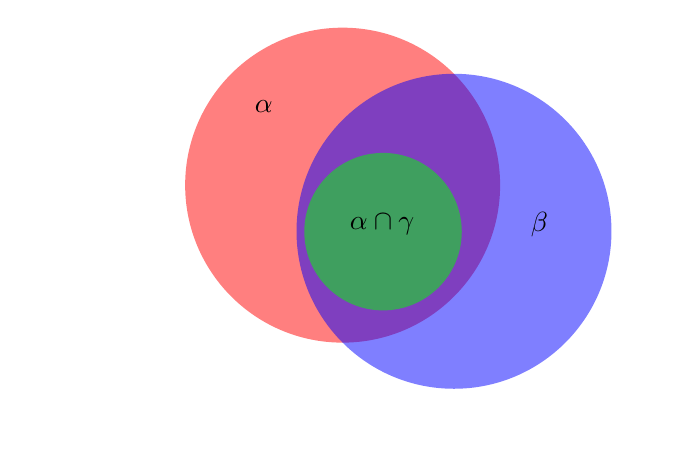
\begin{tikzpicture}
\fill[white](-4,-1) rectangle (4,4);
\fill[opacity=0.5,red] (0,0) ++(90:2) circle (2);
\fill[opacity=0.5,blue] (0,0) ++(45:2) circle (2);
\fill[opacity=0.5,green] (0,0) ++(70:1.5) circle (1);
\node[draw=none] at (-1,3) {$\alpha$};
\node[draw=none] at (2.5,1.5) {$\beta$};
\node[draw=none] at (0.5,1.5) {$\alpha \cap \gamma$};
\end{tikzpicture}}
\item[Mauvaise distribution]:\\
\scalebox{0.5}{
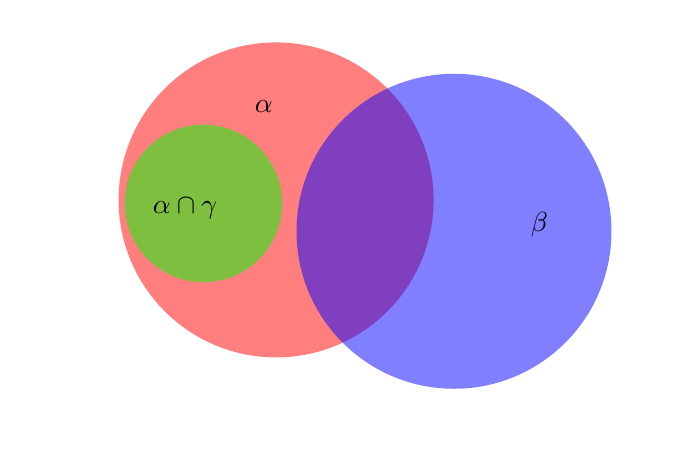
\begin{tikzpicture}
\fill[white](-4,-1) rectangle (4,4);
\fill[opacity=0.5,red] (0,0) ++(115:2) circle (2);
\fill[opacity=0.5,blue] (0,0) ++(45:2) circle (2);
\fill[opacity=0.5,green] (0,0) ++(135:2.5) circle (1);
\node[draw=none] at (-1,3) {$\alpha$};
\node[draw=none] at (2.5,1.5) {$\beta$};
\node[draw=none] at (-2,1.7) {$\alpha \cap \gamma$};
\end{tikzpicture}}
\item[Cas général]:\\
\scalebox{0.5}{
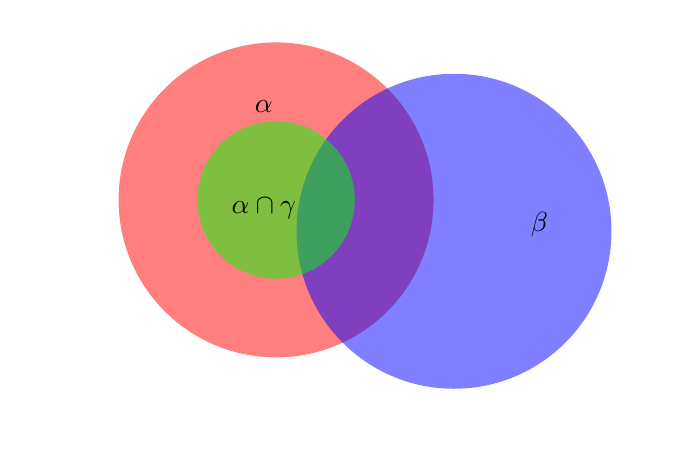
\begin{tikzpicture}
\fill[white](-4,-1) rectangle (4,4);
\fill[opacity=0.5,red] (0,0) ++(115:2) circle (2);
\fill[opacity=0.5,blue] (0,0) ++(45:2) circle (2);
\fill[opacity=0.5,green] (0,0) ++(115:2) circle (1);
\node[draw=none] at (-1,3) {$\alpha$};
\node[draw=none] at (2.5,1.5) {$\beta$};
\node[draw=none] at (-1,1.7) {$\alpha \cap \gamma$};
\end{tikzpicture}}
\end{description}

\section{Système P}
\begin{description}
\item[Réflexivité]:
\begin{description}
\item[Almost all]: $\alpha \almost \alpha$
\item[ensembliste]: $A \Subset A$
\end{description}
\item[Équilibrage à gauche]:
\begin{description}
\item[Almost all]: Si $\models \alpha \Leftrightarrow \beta$ et $\alpha \almost \gamma$ alors $\beta \almost \gamma$
\item[ensembliste]: Si $A = B$ et $A \Subset C$ alors $B \Subset C$
\end{description}
\item[Équilibrage à droite]:
\begin{description}
\item[Almost all]: Si $\alpha \models \beta$ et $\gamma \almost \alpha$ alors $\gamma \almost \beta$
\item[ensembliste]: Si $A \subseteq B$ et $C \Subset A$ alors $C \Subset B$
\end{description}
\item[Coupure]:
\begin{description}
\item[Almost all]: Si $(\alpha \wedge \beta) \almost \gamma$ et $\alpha \almost \beta$ alors $\alpha \almost \gamma$
\item[ensembliste]: Si $(A \cap B) \Subset C$ et $A \Subset B$ alors $A \Subset C$
\end{description}
\item[Monotonie]:
\begin{description}
\item[Almost all]: Si $\alpha \almost \beta$ et $\alpha \almost \gamma$ alors $\alpha \wedge \beta \almost \gamma$
\item[ensembliste]: Si $A \Subset B$ et $A \Subset C$ alors $(A \cap B) \Subset C$
\end{description}
\item[Ou]:
\begin{description}
\item[Almost all]: Si $\alpha \almost \gamma$ et $\beta \almost \gamma$ alors $\alpha \vee \beta \almost \gamma$
\item[ensembliste]: Si $A \Subset C$ et $B \Subset C$ alors $(A \cup B) \Subset C$
\end{description}
\end{description}
\pagebreak
\subsection{Exemple}
Soit:
\begin{description}
\item[$Q$] : être québécoises 
\item[$C$] : être canadiens
\item[$F$] : le fait de parler français 
\item[$A$] : le fait de parler anglais 
\item[$S$] : le fait d'aimer le sirop d'érable
\end{description}
\ \\
\begin{description}
\item[Presque tout les canadiens ne parlent pas le français]: $C \almost \neg F$
\item[Presque tout les québécois parlent le français]: $Q \almost F$
\item[Les québécois aiment le sirop d'érable]: $Q \Rightarrow S \equiv Q \almost S$
\item[Les québécois sont canadiens] $Q \Rightarrow C \equiv Q \almost C$
\end{description}
\ \\
\begin{description}
\item[Presque tout les québécois canadiens parlent le français]\ 
\begin{description}
\item[Nous avons] $Q \almost C$ et $Q \almost F$
\item[Avec la monotonie on obtient] $Q \wedge C \almost F$
\end{description}
\item[Presque tout les québécois canadiens parlent le français ou l'anglais]\ 
\begin{description}
\item[Avec] $Q \wedge C \almost F$
\item[Par ailleurs nous avons] $F \models F \vee A$
\item[Alors via l'équilibrage à droite] $Q \wedge C \almost F \vee A$
\end{description}
\end{description}

\subsection{Caractériser Système P}
Soit la basse de connaissance:
\begin{description}
\item[$\Delta$]
\begin{description}
\item[] $C \Rightarrow \neg F$
\item[] $Q \Rightarrow F$
\end{description}
\item[$W$]
\begin{description}
\item[] $Q \Rightarrow S$
\item[] $Q \Rightarrow C$
\end{description}
\end{description}

\begin{multicols}{2}
[
Pour une formule de type $A \Rightarrow B$ dans $\Delta$ dire si il existe une interprétation qui vérifie $A \Rightarrow B$ et qui satisfait chacune des règles de $\Delta$ et $W$
]
\begin{description}
\item[Pour la formule] $C \Rightarrow \neg F$ est satisfait
\item[$\Delta$]
\begin{description}
\item[] $\corange{C^1} \Rightarrow \neg \cviolet{F^0}$
\item[] $\cblue{Q^0} \Rightarrow \cviolet{F^0}$
\end{description}
\item[$W$]
\begin{description}
\item[] $\cblue{Q^0} \Rightarrow S^s$
\item[] $\cblue{Q^0} \Rightarrow \corange{C^1}$
\end{description}
\end{description}

\begin{description}
\item[Pour la formule] $Q \Rightarrow F$ n'est pas satisfait
\item[$\Delta$]
\begin{description}
\item[] $\corange{C^1} \Rightarrow \neg \cviolet{F^1} \equiv \neg \top \vee \bot$
\item[] $\cblue{Q^1} \Rightarrow \cviolet{F^1}$
\end{description}
\item[$W$]
\begin{description}
\item[] $\cblue{Q^1} \Rightarrow S^s$
\item[] $\cblue{Q^1} \Rightarrow \corange{C^1}$
\end{description}
\end{description}


\end{multicols}

\pagebreak
\chapter{XML}
\pagebreak
uuuuu

\pagebreak

\end{document}

